We have several types of dynamic heuristics based on the fail-first principle:
\begin{itemize}
    \renewcommand{\labelitemi}{-}
    \item \textbf{Minimum domain}. \\
    We choose the decision variable $X_i$ with the \textbf{minimum domain size}, $\textit{min}(|D(X_i)|)$. This strategy is mainly used to minimize 
    the search tree size.
    \begin{example}[title = Minimum domain]
        e.g. Consider the following decision variables order:
        $$\langle X_1, X_2, X_3 \rangle$$
        and their domains:
        $$ X_1 \in \{0, 1, 2, 3\}, X_2 \in \{0, 1, 2\}, X_3 \in \{0, 1\} $$
        We will get a search tree of this size. Of course, changing the order of the decision variables the size would be the same. \vspace{3.5pt}
        \begin{center}
            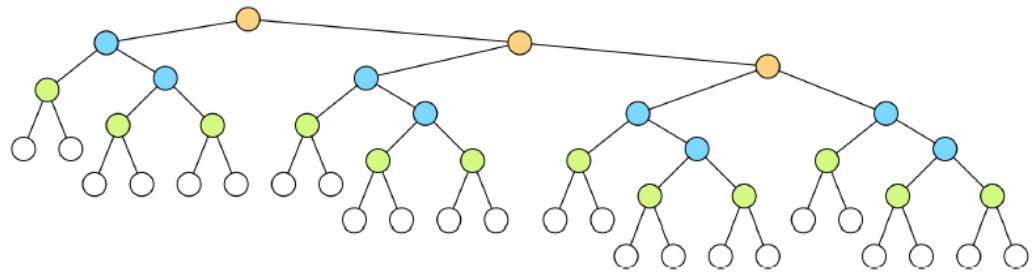
\includegraphics[width = 0.7\textwidth]{img/img18.png}
        \end{center} \vspace{3.5pt}
        Now we consider a total different order:
        $$\langle X_3, X_2, X_1 \rangle$$
        \begin{center}
            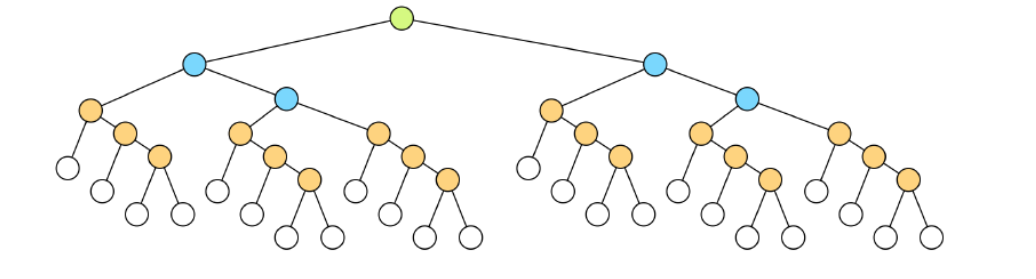
\includegraphics[width = 0.7\textwidth]{img/img19.png}
        \end{center} \vspace{3.5pt}
        The size of the new search tree is the same as before, but we can observe that what really changes is the dimension of the sub-trees. Following a minimum
        domain choice, the propagation effect would be much stronger with the second ordering than the first one.
    \end{example}
    \item \textbf{Most constrained}. \\ 
    We choose the variable involved in the \textbf{most number of constraints}. This strategy is mainly used to maximize the constraint propagation.
    \item \textbf{Combination}. \\ 
    We choose a variable that satisfies \textbf{both} previous strategies. Usually we take the variable that minimizes tha ratio: 
    $$ \frac{\textit{domain size}}{degree} $$
    where:
    \begin{itemize}
        \item $\textit{domain size} \rightarrow$ size of the decision variable domain
        \item $\textit{degree} \rightarrow$ number of constraints in which the variable is involved
    \end{itemize}
\end{itemize}